% fig_blocking.tex  --  Blocking transformation A -> A^{(L)} for FT-MPS
% Requires:  \usepackage{tikz}
%            \usetikzlibrary{calc}
%
% Visualises the coarse-graining step that takes a Matrix Product State
% tensor A = {A^i}_{i=1}^d on Mat_D(C) to the L-blocked tensor A^{(L)}.
% The diagram style follows the tensor-network conventions of the project
% blueprint (small filled circles for tensor dots, thin lines for bonds
% and physical legs, a thin rectangle marking the blocked region).

\begin{figure}[t]
    \centering
    \resizebox{\columnwidth}{!}{%
    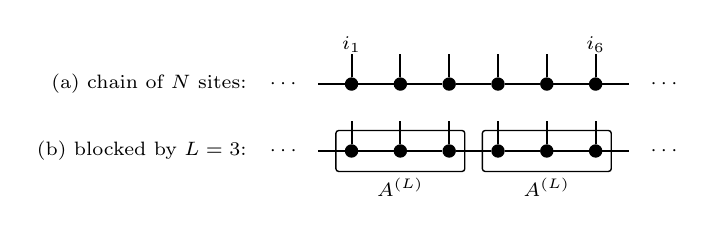
\begin{tikzpicture}[
            baseline=-0.1cm,
            transform shape,
            font=\scriptsize,
            tn dot/.style   ={draw, fill, shape=circle, inner sep=0.055cm},
            tn bond/.style  ={line width=0.5pt},
            tn phys/.style  ={line width=0.7pt},
            tn block/.style ={line width=0.5pt, rounded corners=1pt},
            x=0.62cm
        ]
        %% --- Panel (a): the original chain of N copies of A -------------------
        \begin{scope}[shift={(0,0)}]
            \foreach \i in {0,...,5} {
                    \node[tn dot] (A\i) at (\i,0) {};
                }
            \foreach \i [evaluate=\i as \j using int(\i+1)] in {0,...,4} {
                    \draw[tn bond] (A\i.east) -- (A\j.west);
                }
            \foreach \i in {0,...,5} {
                    \draw[tn phys] (A\i.north) -- ++(0,0.30);
                }
            \draw[tn bond] (A5.east) -- ++(0.55,0);
            \node           at (6.40,0)    {$\cdots$};
            \draw[tn bond] (A0.west) -- ++(-0.55,0);
            \node           at (-1.40,0)   {$\cdots$};
            \node           at (0,0.50)    {$i_1$};
            \node           at (5,0.50)    {$i_6$};
            \node[anchor=east] at (-1.95,0) {(a)\ chain of $N$ sites:};
        \end{scope}
        %% --- Panel (b): the same chain, grouped into L-site blocks ------------
        \begin{scope}[shift={(0,-0.85)}]
            \foreach \i in {0,...,5} {
                    \node[tn dot] (B\i) at (\i,0) {};
                }
            \foreach \i [evaluate=\i as \j using int(\i+1)] in {0,...,4} {
                    \draw[tn bond] (B\i.east) -- (B\j.west);
                }
            \foreach \i in {0,...,5} {
                    \draw[tn phys] (B\i.north) -- ++(0,0.30);
                }
            \draw[tn bond] (B5.east) -- ++(0.55,0);
            \node           at (6.40,0)    {$\cdots$};
            \draw[tn bond] (B0.west) -- ++(-0.55,0);
            \node           at (-1.40,0)   {$\cdots$};
            \foreach \g in {0,1} {
                    \pgfmathsetmacro{\xL}{\g*3 - 0.32}
                    \pgfmathsetmacro{\xR}{\g*3 + 2.32}
                    \pgfmathsetmacro{\xC}{\g*3 + 1}
                    \draw[tn block] (\xL,-0.26) rectangle (\xR,0.26);
                    \node          at (\xC,-0.46) {$A^{(L)}$};
                }
            \node[anchor=east] at (-1.95,0) {(b)\ blocked by $L=3$:};
        \end{scope}
    \end{tikzpicture}%
    }
    \\[0.15em]
    {\footnotesize
        $\displaystyle
            A^{(L)\,(i_1,\ldots,i_L)} \;=\; A^{i_1} A^{i_2} \cdots A^{i_L},
            \qquad
            E_{A^{(L)}} \;=\; {(E_A)}^L$.}
    \caption{Blocking in tensor networks.
        Given an MPS tensor $A$, grouping $L$ consecutive sites yields a single coarse-grained tensor $A^{(L)}$ whose physical index is the composite index $(i_1,\ldots,i_L)$ and whose transfer operator is the $L$-th power ${(E_A)}^L$ of the transfer operator $E_A$ of $A$.
        The spectrum of ${(E_A)}^L$ concentrates onto its dominant eigenvalues as $L$ grows: each block of the resulting canonical form becomes
        \emph{normal} after a finite blocking length and \emph{injective}
        (the matrices of block $k$ span the full algebra
        $M_{D_k}(\C)$)
        after $L = O(D^4)$ further sites, by the quantum Wielandt bound.
        The agent pool reached the single-block injective conjugation autonomously (\cref{eq:equal-MPV-tensor}); the extension to the multi-block regime indicated here was recovered only after the primary references~\cite{Perez-Garcia2007Matrix,Cirac2017Matrixa} were supplied.}\label{fig:blocking}
\end{figure}

